\date{}
\section{Jenis Layanan \textit{Cloud Computing}}
\tab Kata - kata \textit{Cloud}, merujuk kepada suatu simbol model pada dunia IT yang menggambarkan jaringan internet. Tidak semua layanan pada internet yang dapat dikategorikan sebagai cloud computing.\\
\tab Ada setidaknya beberapa persyaratan yang harus terpenuhi oleh suatu layanan berbasis internet untuk dapat diketagorikan sebagai \textit{Cloud computing} yaitu :\\
\begin{enumerate}
\item Layanan tersebut harus bersifat on demand ; kebebasan dalam memilih salah satu layanan yang disediakan oleh provider kepada pengguna dan pengguna membayarnya berdasarkan apa yang mereka gunakan.
\item Layanan bersifat elastis / scalable ; elastis suatu layanan berbasis internet harus dapat mengakomodasi dan memenuhi permintaan serta kebutuhan pengguna kapan saja
\item Layanan yang tersedia sepenuhnya dikelola oleh provider sedangkan pengguna hanya membutuhkan koneksi internet untuk menggunakan layanan tersebut.
\item Layanan tersebut harus terukur ; sumber daya cloud yang tersedia secara transparan harus dapat dioptimasi dan terukur oleh pengguna untuk menjadi acuan dalam memenuhi kebutuhan pengguna.
\end{enumerate}
\tab Berdasarkan layanan, cloud computing terbagi dalam 7 tingkatan yang biasanya digunakan oleh pengguna yaitu \textit{software as a service, utility computing, web service, platform layanan, management service provider, e-commerce, dan integrated network}.\\
\section{\textit{Software as Service}}
\tab \textit{Software as Service} merupakan evolusi lanjutan dari konsep ASP (\textit{Application Service Provider}). \textit{Software as Service} adalah istilah terhadap software atau aplikasi tertentu berbasis internet yang ditawarkan oleh provider kepada pengguna. Dalam hal ini, provider sebagai pemegang license atas software tersebut hanya memberikan service atau layanan kepada pengguna untuk menggunakannya sesuai kebutuhan pengguna dengan demikian menghilangkan kerumitan dalam hal pemeliharaan software, operasional dan support. License, maintenance, support, tingkat kenyamanan dan keamanan atas software tersebut sepenuhnya menjadi tanggung jawab dari provider.\\
\tab Kata – kata \textit{Software} merujuk kepada perangkat lunak suatu system, dimana perangkat lunak pada umumnya memiliki beragam karakteristik. Tidak semua perangkat lunak yang beredar di pasaran dapat dikategorikan sebagai \textit{SaaS}, ada beberapa karakteristik yang harus terpenuhi :\\
\begin{itemize}
\item Berbasis internet ; software harus dapat diakses dan dikelola oleh pengguna melalui media internet.
\item Software bersifat terpusat atau ter-sentral sehingga memungkinkan pengguna untuk mengaksesnya darimana dan kapan saja.
\item Memiliki fasilitas untuk meng-update atau meng-upgrade secara terpusat sehingga pengguna tidak perlu download patch atau upgrade di masing – masing komputer.
\item Aplikasi yang ditawarkan oleh provider bersifat \textit{multi tenant}
\end{itemize}
\textit{Software as Service} menawarkan beberapa keuntungan kepada pengguna dibanding dengan model aplikasi desktop:
\begin{itemize}
\item Model rancangan dan distribusi software lebih menarik dan harga terjangkau karena memungkinkan membagi satu aplikasi kepada ratusan perusahaan dan berjalan dalam lingkungan sistem biasa. Secara luas memberikan improvisasi kepada model client /server.
\item Biaya pemakaian bandwidth untuk menjaga tingkat konektivitas relatif terjangkau.
\item Mempermudah pengguna untuk melakukan migrasi aplikasi, dengan menghilangkan sisi pembayaran license software dan keharusan membayar upgrade.
\item Meningkatkan produktivitas bagi pengguna
\end{itemize}
Gambar 3.1 menjelaskan ketika provider mempublikasikan suatu layanan \textit{SaaS} di internet dan satu atau beberapa pengguna saling menggunakannya secara bersama – sama atau on demand di dalam internet
\begin{center}
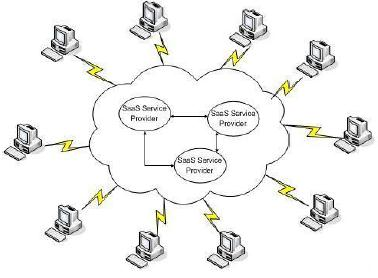
\includegraphics[scale=1]{Gambar31.jpg} \\
\textbf{Gambar 3.1}
\end{center}
\tab Implementasi \textit{cloud computing} dapat diterapkan pada jaringan yang bersifat public atau jaringan yang bersifat private. Jaringan yang bersifat public adalah suatu jaringan yang dapat diakses dan digunakan secara umum oleh setiap orang selama orang tersebut terkoneksi dengan internet sedangkan jaringan yang bersifat private adalah suatu jaringan yang hanya dapat diakses dan digunakan oleh orang – orang tertentu meskipun melalui koneksi internet.\\
\tab Ketika cloud computing diimplementasikan ke dalam jaringan public, maka seluruh sumber daya atau textit{resources} dari aplikasi sepenuhnya berada internet. Layanan textit{SaaS} yang bersifat public sering kita jumpai dalam bentuk aplikasi web atau web services. Ketika provider meletakkan seluruh sumber daya atau \textit{resources} dari aplkasi ke dalam internet tetapi hanya beberapa orang yang dapat menggunakannya maka layanan textit{SaaS} tersebut bersifat private.\\
\tab textit{SaaS} yang ditawarkan provider kepada pengguna baik melalui jaringan public maupun jaringan private pada dasarnya mempunyai satu karakteristik yang sama yaitu mudah diakses dan berskala luas (upgrade aplikasi, modifikasi aplikasi disesuaikan dengan kebutuhan dan keinginan pengguna).
\tab Berbagai textit{SaaS} yang dibuat oleh provider sering disebut dalam berbagai versi yaitu versi berbasis web, textit{on demand} dan sebagainya. Apapun versi yang dibuat oleh provider, yang diperlukan oleh pengguna adalah koneksi internet untuk dapat menggunakan textit{SaaS} tersebut.
\tab Metodologi pengembangan dari textit{SaaS} memiliki kesamaan dengan pengembangan software desktop baik dari sisi kemampuan aplikasi diakses dalam skala besar, tingkat keamanan dan aplikasi yang nyaman digunakan oleh pengguna. Beberapa faktor keberhasilan dalam implementasi dan pengembangan textit{SaaS} yaitu :\\
\begin{itemize}
\item Efisiensi sumber daya komputer : textit{SaaS} memiliki kemampuan memaksimalkan penggunaan sumber daya komputer seperti pemakaian memory dan bandwidth secara bersamaan, penggunaan database berskala besar untuk berbagai pengguna di berbagai lokasi yang berbeda dalam waktu bersamaan.
\item Optimasi data dan textit{multi tenant} : textit{SaaS} memiliki kemampuan untuk memilah data – data dan menseleksi data – data berdasarkan kepemilikan pengguna secara bersamaan dalam satu aplikasi ( textit{multi tenant} ).
\item Fleksibel aplikasi : textit{SaaS} memiliki tingkat fleksible yang tinggi dan memungkinkan pengguna memodifikasi aplikasi sesuai kebutuhan pengguna.
\end{itemize}
Berdasarkan ketiga faktor keberhasilan tersebut dan membandingkan berbagai aplikasi berbasis \textit{SaaS} yang ditawarkan oleh provider, maka kita dapat mengelompokkan berdasarkan kategori seperti yang terdapat pada gambar 3.1.1\\
\begin{center}
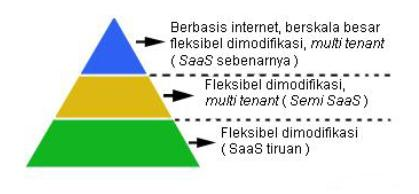
\includegraphics[scale=1]{Gambar311.jpg} \\
\textbf{Gambar 3.1.1}
\end{center}
\tab Secara arsitektur, \textit{SaaS} memiliki kesamaan dengan SOA ( textit{Service Oriented Architecture} ) yang dimiliki oleh software desktop, \textit{SaaS} memiliki dua lapisan tambahan yang tidak dimiliki oleh software desktop. Perbedaan tersebut adalah :\\
\begin{enumerate}
\item \textit{Meta data services} : lapisan ini memberikan kemudahan bagi pengguna untuk melakukan modifikasi terhadap aplikasi baik dari sisi memodifikasi tampilan aplikasi, memodifikasi fungsional aplikasi agar sesuai dengan konsep dan aturan bisnis di perusahaan pengguna, dan memodifikasi pengaturan atau kontrol terhadap data termasuk migrasi data yang tersedia. Kemudahan dalam memodifikasi aplikasi sepenuhnya di tangan pengguna.
\item \textit{Security services} : lapisan keamanan ini mendelegasikan setiap pengguna untuk bertanggung jawab sepenuhnya terhadap apapun yang dibuat di dalam aplikasi ini termasuk mendelegasikan keamanan password dari masing – masing \textit{user account ( tenant )} yang dibuat oleh pengguna. Meskipun provider sebagai pemilik sepenuhnya atas \textit{SaaS} yang ditawarkan, \textit{SaaS} memberikan kemampuan kepada pengguna untuk membuat aturan bisnis terhadap aplikasi, dan kontrol akses terhadap aplikasi sesuai keinginan pengguna.			
\end{enumerate}
Berdasarkan gambaran umum dari sisi pengguna, SaaS yang ditawarkan oleh provider terkesan sebagai satu aplikasi dalam satu database yang khusus diberikan oleh provider kepada pengguna. Gambaran umum dari sisi pengguna seperti ini tidak sepenuhnya salah karena aplikasi yang berbasis SaaS memiliki tiga model yang masing – masing model tersebut disesuaikan dengan keinginan dan kebutuhan pengguna.\\
\tab Pada gambar 3.1.2 menjelaskan tiga model berbasis SaaS yang umum ditawarkan oleh provider.\\
\begin{center}
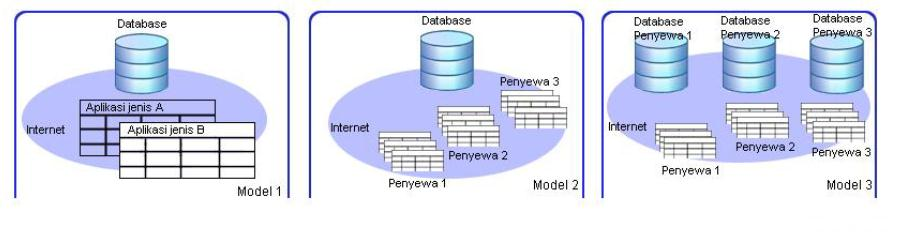
\includegraphics[scale=0.8]{Gambar312.jpg} \\
\textbf{Gambar 3.1.2}
\end{center}
Gambar 3.1.2 pada \textit{SaaS} model 1 menjelaskan pengguna atau penyewa \textit{SaaS} memiliki beberapa aplikasi yang berbeda jenis tetapi hanya memiliki satu database yang di share atau digunakan bersama – sama untuk beragam aplikasi yang dibuat oleh pengguna atau penyewa. Pengguna atau penyewa SaaS cukup melakukan modifikasi aplikasi, mengubah skala aplikasi melalui koneksi internet. \textit{SaaS} model 1 ini pada umumnya ditawarkan oleh provider dalam bentuk virtualisasi server ( VPS ) dan bersifat private.\\
\tab Pada \textit{SaaS} model 2 menjelaskan beberapa penyewa atau pengguna \textit{SaaS} memiliki aplikasi yang terpisah dan berbeda – beda tetapi mengakses database yang sama atau satu database digunakan secara bersama – sama oleh beragam aplikasi dan beragam penyewa. \textit{SaaS} model 2 ini pada umumnya ditawarkan oleh provider dalam bentuk aplikasi berbasis web atau \textit{web services}, salah satu contoh \textit{SaaS} model 2 adalah \textit{email}, terkadang demi menarik konsumen untuk menggunakan \textit{SaaS} model 2, provider memberikannya secara gratis.\\
\tab Pada SaaS model 3 menjelaskan beberapa penyewa \textit{SaaS} memiliki masing – masing aplikasi yang berbeda termasuk database yang berbeda dan bersifat private. Satu penyewa memiliki beragam aplikasi tetapi memiliki satu database private yang digunakan untuk aplikasi penyewa itu sendiri. Masing – masing penyewa terpisah secara mandiri baik dari aplikasi maupun secara database.
\textit{SaaS} model 3 ini adalah model gabungan dari model 1 dan model 2 yang memang dibangun dan dibuat oleh provider \textit{SaaS} untuk memenuhi kebutuhan pengguna. Salah satu contoh \textit{SaaS} model 3 adalah aplikasi \textit{office suite} berbasis web.\\
\tab Kesimpulan dari \textit{SaaS ( Software as a Service )} : \textit{SaaS} merupakan evolusi dari pengembangan software dimana aplikasi tersebut diletakkan di cloud atau internet. Aplikasi tersebut tersedia di internet atau cloud sehingga pengguna tidak perlu melakukan instalasi atau menjalankan aplikasi tersebut di masing – masing komputernya. Sebagai hasilnya pengguna terbebaskan dari urusan maintenance aplikasi. Oleh provider \textit{SaaS} ditawarkan sebagai \textit{pay as you use service} , artinya pembayaran atas software atau aplikasi termasuk license didalamnya tidak diperlukan, pembayaran hanya dilakukan ketika aplikasi digunakan dan biaya tersebut dihitung berdasarkan periode biasanya per bulan, per tahun.\\
\tab Untuk provider software atau yang dikenal dengan istilah \textit{software house}. \textit{SaaS} memberikan keuntungan karena aplikasi atau software yang dibuatnya terlindungi dari pembajakan software dan keuntungan dari kegunaan aplikasi yang diinginkan oleh pengguna. Pada umumnya mereka ( \textit{software house} ) meletakkan aplikasinya di dalam server berbasis cloud atau lingkungan hosting. Lingkungan hosting merupakan suatu platform yang menjadi landasan untuk aplikasi berjalan, karena itu hosting identik dengan layanan \textit{PaaS ( Platform as a service )}.\\
\tab Dari kedua sisi ini, \textit{SaaS} merupakan evolusi teknologi software yang dapat ditingkatkan menjadi \textit{multi tenant} atau banyak pengguna mengakses sumber daya yang sama. Layanan \textit{SaaS} identik dengan layanan \textit{PaaS}. \textit{PaaS} merupakan istilah dari \textit{platform as a service}, dimana pada \textit{SaaS} terfokus pada aplikasi sedangkan aplikasi itu sendiri merupakan suatu platform dan membutuhkan platform tertentu.\\
\tab Implementasi \textit{SaaS} tidak dapat berjalan dengan baik jika tidak didukung dengan infrastruktur penunjang yang solid dan baik. Dengan alasan pengembangan bisnis, jika infrastruktur penunjang sudah solid dan kuat, terkadang provider dapat menawarkannya kepada pengguna. Layanan infrastruktur ini dikenal sebagai \textit{utility computing}.\\

\section{\textit{Utility Computing}}
\tab \textit{Cloud computing} tidak hanya melibatkan sisi aplikasi atau perangkat lunak saja, tetapi juga melibatkan perangkat keras atau hardware dan sumber daya penunjang. Seperti yang telah kita ketahui layanan \textit{SaaS} lebih berfokus pada aplikasi atau perangkat lunak, sedangkan pada infrastruktur sebagai layanan \textit{utility computing}. Layanan \textit{utility computing} dikemas oleh provider dalam bentuk teknologi virtualisasi dan dikenal sebagai layanan \textit{IaaS ( Infrastructure as a Service )}. Pada gambar 3.2 menjelaskan arsitektur komputer secara traditional atau standalone.\\
\begin{center}
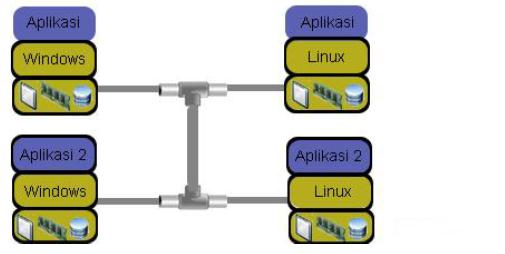
\includegraphics[scale=1]{Gambar32.jpg} \\
\textbf{Gambar 3.2}
\end{center}
\begin{center}
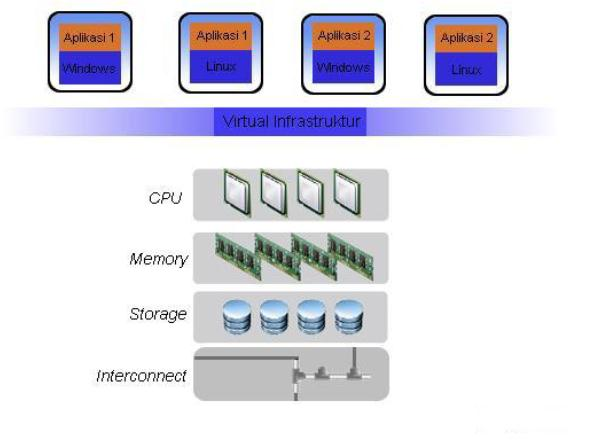
\includegraphics[scale=1]{Gambar321.jpg} \\
\textbf{Gambar 3.2.1}
\end{center}
Pada gambar 3.2.1 masing – masing aplikasi dan masing – masing sistem operasi ( windows dan linux ) menggunakan sumber daya komputer yang sama. Sistem operasi pada gambar tersebut bukanlah sesuatu yang special sebagai peranan utama dalam infrastruktur virtualisasi. Sistem operasi hanya sebagai perantara untuk dapat menjalankan virtual mesin.\\
\tab Peranan utama dalam infrastruktur virtualisasi adalah \textit{hypervisor}. \textit{Hypervisor} merupakan software yang menggantikan fungsi utama dari operating sistem ketika operating sistem selesai menjalankan virtual mesin. \textit{Hypervisor} diasumsikan sebagai \textit{virtual machine manager}, yang didesign untuk dapat menjalankan virtual mesin lainnya dan menjalankan sistem operasi dari awal seperti ketika komputer dinyalakan. Untuk lebih jelas mengenai arsitektur virtualisasi dapat dilihat pada bab 2.\\
\tab Dengan teknologi virtualisasi, pengguna atau penyewa \textit{IaaS} dapat mengakses dan menggunakan seluruh sumber daya komputer dan seluruh sumber daya lainnya yang tersedia di dalam \textit{cloud} sesuai kebutuhan dan keinginan pengguna.\\
\tab Teknologi virtualisasi memungkinkan untuk diimplementasikan berbagai aplikasi dengan tujuan yang beragam dalam 1 platform atau aplikasi, seperti \textit{storage computing, image manipulation, parallel processing, content distribution}, aplikasi web dan sebagainya. Dalam menawarkan layanan \textit{IaaS} kepada pengguna atau penyewa, provider membagi \textit{IaaS} dalam beberapa kategori layanan yaitu :\\
\begin{enumerate}
\item Layanan penyimpanan dan komputasi virtual : yaitu VMware rental, penyimpanan online ( \textit{Online Storage} ).
\item Layanan kustomise : yaitu \textit{server template}.
\item Layanan automasi dan control : yaitu \textit{automation}.
\item Layanan penghubung : yaitu \textit{remote control}, web 2.0.
\item Layanan monitoring : yaitu monitor secara fisik objek yang diinginkan ( posisi koordinat bumi, peta, kamera ).
\item Layanan optimasi objek : yaitu virtualisasi network, virtualisasi penyimpanan, virtualisasi server.
\item Layanan pengukuran objek : yaitu pengukuran fisik suatu objek.
\item Layanan integrated dan kombinasi objek : yaitu \textit{load balance}.
\item Layanan security : yaitu enkripsi data penyimpanan, VM isolation, VLAN dan SSL/SSH.		
\end{enumerate}
Jantung dari teknologi cloud computing adalah virtualisasi, dimana virtualisasi dapat diterapkan pada 2 sisi yaitu pada sisi provider dan sisi pengguna ( desktop pengguna ) seperti pada gambar 3.2.2.\\
\begin{center}
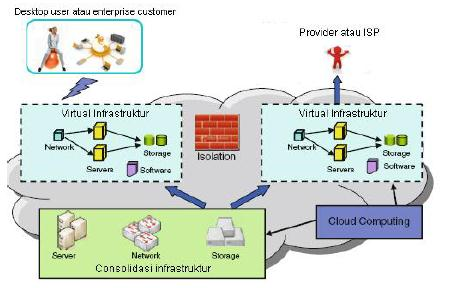
\includegraphics[scale=1]{Gambar322.jpg} \\
\textbf{Gambar 3.2.2}
\end{center}
\tab Beberapa software virtualisasi seperti VMware, citrix dan sebagainya mempunyai kemampuan untuk menciptakan fungsi lain yang disebut sebagai \textit{virtual desktop interface} ( VDI ).
\tab \textit{Virtual desktop interface} ( VDI ) menciptakan session untuk client atau user di dalam server, dan mengirimkan virtual PC tersebut kepada client atau user sehingga user dapat berinteraksi dengan server seakan client atau user tersebut berada di dalam server itu sendiri. Perbedaan yang cukup signifikan antara software remote dengan virtual PC :\\
\begin{itemize}
\item \textit{Software remote} adalah software yang dapat digunakan untuk melakukan pengendalian jarak jauh ke satu komputer atau satu server dalam satu koneksi hanya untuk satu user atau client. Jika satu komputer atau satu server diakses oleh lebih dari dua user maka komputer atau server yang diakses secara remote akan memutuskan salah satu koneksi dari dua koneksi yang terjadi.
\item \textit{Software remote} hanya software atau aplikasi penghubung ke komputer lain dan tidak dapat berfungsi untuk menciptakan komputer di dalam komputer itu sendiri.	
\end{itemize}
\tab Dalam gambar 3.2.2 user terkoneksi dan menggunakan layanan \textit{IaaS} ke server provider melalui \textit{virtual desktop interface} ( VDI ) di internet. Sedangkan pada sisi provider, provider melakukan konfigurasi server melalui jalur yang sama ( VDI ) di internet. Untuk dapat menerapkan teknologi virtualisasi di cloud maka server yang sudah diimplementasikan teknologi virtualisasi diletakkan di dalam cloud ( private cloud atau public cloud ) sebagai back end infrastruktur.\\
\tab Dari prespektif ini, sumber daya teknologi virtualisasi atau \textit{virtual resources} di dalam cloud diasumsikan sebagai sumber daya komputer yang bersifat independent atau mandiri termasuk lokasi dari sumber daya itu sendiri.\\
\tab Infrastruktur juga memegang peranan utama untuk memastikan semua komponen bekerja dengan baik dalam kondisi multi tenant dan bertanggung jawab terhadap segala aktifitas yang terjadi. Seperti yang sudah dijelaskan sebelumnya bahwa teknologi virtualisasi merupakan jantung utama dari \textit{cloud computing}, dimana teknologi virtualisasi hanyalah berupa aplikasi atau software. Teknologi virtualisasi tidak dapat berjalan sempurna tanpa didukung dengan infrastruktur yang baik dan solid. Teknologi virtualisasi memungkinkan untuk diterapkan \textit{redundancy, replication atau cluster, dan workload balancing.}\\
\begin{center}
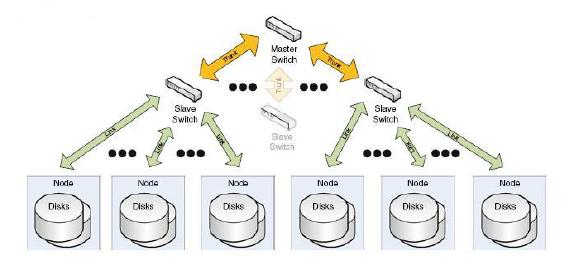
\includegraphics[scale=1]{Gambar323.jpg} \\
\textbf{Gambar 3.2.3}
\end{center}
\section{Web Service}
\tab Kemampuan unik dari \textit{web service} adalah membantu para programmer untuk membuat suatu aplikasi berbasis web dengan fungsi lain di atas platform web itu sendiri. Dalam beberapa kasus, coding – coding yang dihasilkan oleh programer yang menyewa layanan ini membagikan ( \textit{share} ) dan dikumpulkan dalam penyimpanan data yang dikelola oleh provider.\\
\tab Pada kasus lainnya, aplikasi – aplikasi tersebut dalam bentuk \textit{application programming interface} ( API ), plug-ins, atau full aplikasi yang dapat diintegrasikan dengan aplikasi berbasis web. Semua aplikasi tersebut tidak hanya tersedia hanya untuk kalangan programer yang menyewa layanan ini, tetapi juga untuk para programer pada umumnya.
\tab Pada layanan selain \textit{web service}, provider hanya bertanggung jawab untuk menjaga dan mengelola infrastruktur penunjang. Sedangkan pada layanan \textit{web service} ini, secara umum provider berusaha untuk menyediakan dan memberikan sekumpulan tools atau aplikasi penunjang yang lengkap yang dapat mempermudah para programer aplikasi web untuk membuat aplikasi. Kolaborasi dari aplikasi penunjang pada layanan ini diperoleh karena kerja sama antar partner bisnis dimana partner bisnis tersebut merupakan programmer atau institusi independent yang membangun aplikasi berbasis web.\\
\tab Bagi para programer, layanan ini merupakan pendekatan dan cara termudah dalam mendesign, dan membuat aplikasi berbasis web dengan komitmen pembayaran yang lebih murah dan terjangkau pada hardware dan software. Biaya yang dikeluarkan atas layanan ini masih terjangkau dibandingkan dengan menggunakan biaya atas jasa pembuatan aplikasi dan biaya maintenance.\\
\tab Layanan ini membantu programer untuk fokus kepada mendesign dan membuat aplikasi berbasis web. Ada dua faktor yang menentukan suatu aplikasi berbasis web dikategorikan sebagai buruk atau baik yaitu penampilan dan bobot kualitas isinya ( \textit{content} ).\\
\tab Penampilan membutuhkan keahlian dan kreatifitas dalam mendesign semua komponen, elemen serta style atau gaya design. Penampilan dari aplikasi berbasis web merupakan faktor penentu banyak orang yang berinteraksi dalam aplikasi tersebut, sedangkan content atau kualitas isinya yang mengelola informasi harus mudah dimengerti dan mudah dibaca oleh user.\\
\tab Peranan utama dari web service terletak pada \textit{application programming interfaces} ( API ) yang melekat pada \textit{web service}. Menggunakan \textit{web service} berbasis API identik dengan mengakses protocol berbasis SOAP ( \textit{Simple Object Access Protocol} ). Model pemograman API seperti mengakses dan menggunakan aplikasi di luar dari lingkungan seharusnya aplikasi tersebut berada, dimana lokasi data dan layanan protocol aplikasi tersebut berbeda lokasi.\\
\tab Karena aplikasi dengan lokasi data termasuk protocolnya terpisah dan berbeda lokasi, maka menjadi tanggung jawab programer untuk memastikan aplikasi berbasis API dapat digunakan.\\
\tab Pendekatan model pemograman API sudah digunakan dan diterapkan oleh banyak provider besar, beberapa contoh provider yang menerapkan model ini adalah google, facebook, dan Microsoft. Untuk pembahasan lebih lanjut mengenai penerapan yang dilakukan oleh provider ini dapat dilihat pada bab 4.\\
\tab Pada dasarnya web service merupakan aplikasi berbasis web yang mengkombinasikan antara data dan fungsi aplikasi dari berbagai lokasi. Aplikasi itu sendiri hanya merupakan sekumpulan kode – kode program yang diletakkan pada lokasi yang berbeda dari data dan protocol yang digunakan.\\
\tab Tiga faktor yang menjadi peranan utama dalam kesuksesan layanan web service adalah :
\begin{enumerate}
\item Menyediakan sarana berbasis aplikasi yang memungkinkan para programer untuk membangun atau membuat suatu aplikasi.
\item Menyediakan sarana bagi user atau pengguna untuk dapat menggunakan aplikasi yang memberikan efek manfaat atau kegunaan sesuai kebutuhan pengguna dan memiliki koneksitas berskala luas.
\item Menyediakan sarana bagi pengguna atau programer untuk dapat melakukan maintenance secara mandiri dan mengintegrasikan dengan aplikasi lainnya.
\end{enumerate}
Pada gambar 3.3, merupakan arsitektur dari \textit{web service}\\
\begin{center}
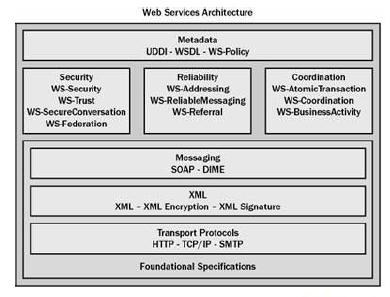
\includegraphics[scale=1]{Gambar33.jpg}\\
\textbf{Gambar 3.3}
\end{center}
\tab Seperti yang telah dibahas pada awal subbab 3.3, \textit{web service} menggunakan platform \textit{application programming interface} ( API ). Prinsip dasar dari API identik dengan SOAP ( simple object application protocol ) seperti pada gambar 3.3 didalam arsitektur web service terdapat lapisan yang disebut dengan SOAP.\\
\tab SOAP merupakan protocol yang bertanggung jawab terhadap pertukaran data atau informasi yang secara desentralisasi dan terdistribusi. Protocol yang digunakannya adalah http ( \textit{hypertext transfer protocol} ).\\
\tab Peranan SOAP di dalam teknologi \textit{web service} adalah sebagai protocol yang melakukan pemaketan pesan – pesan ( \textit{messages} ) yang digunakan secara bersama oleh aplikasi – aplikasi penggunanya. Spesifikasi pemaketannya sendiri tidak lebih dari sebuah amplop biasa berbasis XML untuk sebuah informasi yang akan dikirim, serta sekumpulan aturan bagi translasi aplikasi dan tipe – tipe data dari platform yang spesifik.\\
\tab Pesan dari SOAP adalah sebuah dokumen XML yang terdiri atas beberapa element :\\
\begin{enumerate}
\item Elemen \textit{envelope} : elemen yang mengidentifikasi dokumen XML sebagai sebuah pesan SOAP.
\item Elemen \textit{header} : elemen ini bersifat opsional, berisi informasi header.
\item Elemen \textit{body} : berisikan panggilan dan merespon informasi.
\item \textit{Fault} elemen : elemen yang bersifat opsional, berisikan pesan kesalahan yang terjadi pada waktu proses.

\end{enumerate}
Contoh bentuk dari dokumen XML seperti pada gambar 3.3.1.\\
\begin{center}
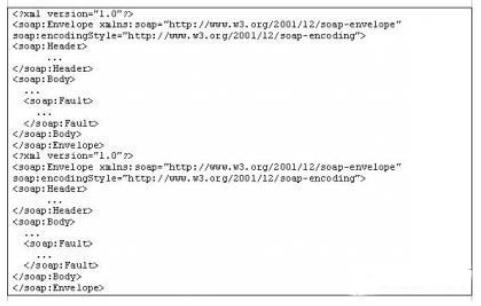
\includegraphics[scale=1]{Gambar331.jpg}\\
\textbf{Gambar 3.3.1}
\end{center}
\tab Pada gambar 3.3.2 secara umum \textit{web service} terbentuk dari semua komponen yang bersifat abstrak, bervariasi dan dinamis. Semua komponen tersebut saling terkait secara berkesinambungan dan menghasilkan suatu aplikasi yang \textit{user friendly} atau mudah digunakan bagi pengguna. Komponen – komponen tersimpan secara terpusat dalam lokasi yang dikenal sebagai portal.\\
\tab Beberapa provider seperti google, Microsoft dan facebook memperluas jangkauan layanan ini dalam berbagai device atau alat mobile untuk memperluas jangkauan penyebaran informasi.\\
\begin{center}
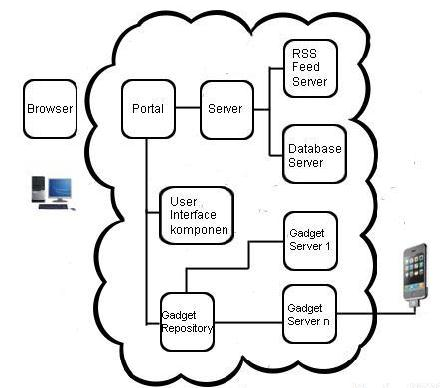
\includegraphics[scale=1]{Gambar332.jpg}\\
\textbf{Gambar 3.3.2}
\end{center}
\section{\textit{E Commerce}}
\tab Ketika aplikasi berbasis web menjadi salah satu teknologi penunjang yang menghubungi pelanggan, rekan bisnis dan karyawan kepada aplikasi perusahaan melalui jaringan internet, \textit{e commerce} berkembang pesat menjadi suatu aplikasi berbasis web yang mengakomodasi berbagai kebutuhan pelanggan.\\
\tab \textit{E commerce} yang merupakan istilah dari perdagangan berbasis elektronik mengharuskan perusahaan untuk melakukan integrasi antara sisi internal dan eksternal proses bisnis mereka kepada era teknologi dan informasi berbasis aplikasi web.\\
\tab Ketika perusahaan melibatkan proses bisnis mereka melalui jaringan intranet, extranet kemudian melalui jaringan internet, \textit{e commerce} berhasil menekan sisi biaya, menjangkau pemasaran lebih luas dan meningkatkan hubungan bisnis mereka kepada rekan bisnis.\\
\tab Seiring dengan berkembangnya \textit{e commerce}, perusahaan berhasil meraih keuntungan bisnis, salah satu contoh perusahaan yang berhasil meraih keuntungan terbesar melalui \textit{e commerce} adalah Amazon.com.\\
\tab Bagaimanapun juga keberhasilan yang diraih oleh \textit{e commerce} melalui jaringan internet memiliki beberapa resiko finansial dalam bertransaksi. Atas dasar ini subbab dari 3.4 lebih terfokus pada sisi arsitektur dari provider keamanan transaksi dan sisi skalabilitas aplikasi web.\\
\tab Melihat pada resiko keamanan secara finansial dalam bertransaksi \textit{e commerce}, banyak industri atau perusahaan yang meng-integrasikan aplikasi berbasis web mereka dengan provider keamanan transaksi atau perusahaan yang berfokus pada keamanan transaksi.\\
\tab Untuk mempermudah dalam memahami sisi arsitektur dan skalabilitas aplikasi web untuk diintegrasikan dengan provider keamanan transaksi, maka diambil salah satu contoh provider security ( keamanan transaksi ) yaitu paypal.\\
\tab Seperti yang telah dibahas arsitektur aplikasi berbasis web pada subbab 3.3, arsitektur dari paypal adalah \textit{web service} atau aplikasi web berbasis SOAP (\textit{ simple object access protocol }), yang memberikan skalabilitas untuk mengintegrasikan dan mengkombinasikan \textit{client side} dan \textit{server side}.
\begin{center}
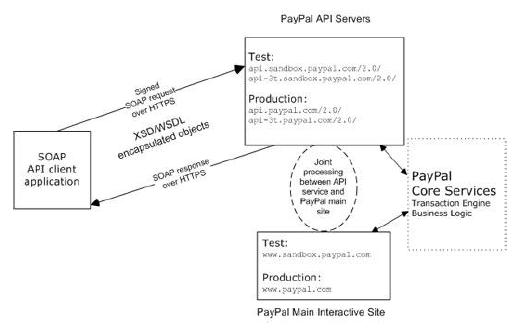
\includegraphics[scale=1]{Gambar34.jpg}\\
\textbf{Gambar 3.4}
\end{center}
\tab Pada gambar 3.4 dalam model OOP ( \textit{object oriented programming} ) ini, interface ke SOAP request/response merupakan objek dari bahasa pemograman native yang dapat diintegrasikan ke SOAP dari aplikasi web. Paypal menyediakan file – file WSDL dan XSD yang secara spesifik merupakan struktur message atau pesan dari paypal, isi data, dan layanan ( service ) API dari paypal.\\
\tab Aplikasi bisnis termasuk data didalamnya berada dan berjalan dalam property objek ini. Untuk mengirim dan menerima data dapat dilakukan dengan metode pemanggilan objek tersebut. Objek SOAP client menangani permintaan membentuk SOAP baru dan mengirimkan kepada layanan paypal, kemudian layanan paypal memberikan umpan balik atau \textit{feedback} ke objek SOAP client.\\
\tab Skema dan prinsip dasar dari web service paypal adalah \textit{eBay business language} ( eBL ). Dan inti komponen yang diperlukan dalam mengintegrasikan aplikasi web ke layanan paypal adalah API paypal yaitu file – file WSDL dan XSD.\\
\tab Secara mendasar konsep dan terminology dari API paypal adalah :\\
\begin{itemize}
\item \textit{API calls} : Layanan API paypal, melalui fungsi objek ini, perusahaan bisnis atau organisasi dapat melakukan pembayaran via online, pencarian transaksi, pengembalian ( refund ) pembayaran, melihat informasi transaksi dan beberapa fungsi lain yang diperlukan oleh dunia bisnis.
\item \textit{API certificate} : Merupakan \textit{API signature}, paypal akan memberikan satu digital sertifikat yang bersifat unik yang dapat didownload dari website paypal. Fungsi ini akan digunakan oleh setiap komputer user yang akan mengakses, dan sertifikat ini akan me-\textit{encrypt} data ketika objek \textit{API calls} dipanggil atau digunakan melalui protocol https dan mengirimnya ke API server.
API sertifikat ini sangat cocok diterapkan ke \textit{web server}.
\item \textit{API signature} : Merupakan \textit{API certificate}, paypal akan memberikan satu \textit{digital signature} ( satu baris dari text atau metode pengacakkan hash ) yang dapat diperoleh dengan mengcopy \textit{API calls} nya. Sebagai fungsi alternative dari \textit{API certificate}.
\textit{Digital signature, API username}, dan \textit{API password} semuanya merupakan bagian yang disebut sebagai tiga token \textit{authentication}.
\item \textit{API username }dan
\textit{API password} : Di \textit{generate} atau dibuat oleh paypal, yang meidentifikasikan nama rekening dan password yang secara special digunakan untuk \textit{API calls}.
Selalu melibatkan username dan password setiap kali menggunakan dan memanggil\textit{ API call.}
\textit{API username }dan \textit{API password} berbeda dengan penggunaan ketika login ke website paypal. Pada website paypal, untuk login yang diperlukan adalah email dan password yang berbeda dari \textit{API username} dan \textit{API password.}
\item \textit{Subject authorization} : Sebagai indikator bagi \textit{API call}, yang merupakan informasi rekening \textit{API call} itu dibuat.
Ini merupakan aspek yang dibuat oleh provider paypal sebagai authorisasi.
\item \textit{First-party access} : Perusahaan atau organisasi diberikan kebebasan untuk membuat \textit{API call} dari server miliknya ke server paypal.
Perusahaan diperbolehkan untuk memiliki \textit{API certificate }atau \textit{API signature, username} dan \textit{password} sebagai miliknya.
Sebagai contoh :
Programer dari perusahaan \textit{merchant}, memperoleh file \textit{API certificate} yang diterbitkan oleh paypal. Oleh programmer tersebut dibuatkan \textit{API call} untuk perusahaannya dari server milik perusahaannya.
\end{itemize}
Pada gambar 3.4.1 merupakan diagram dari \textit{SOAP request.}
\begin{center}
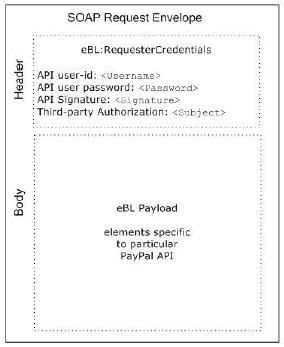
\includegraphics[scale=1]{Gambar341.jpg} \\
\textbf{Gambar 3.4.1}
\end{center}
\tab Kesimpulan dari \textit{ecommerce} : pondasi dari \textit{ecommerce} adalah tekonologi \textit{web service} yang memiliki skalabilitas untuk diintegrasikan dengan aplikasi lain yang berbeda lokasi dan berbeda provider. Karena \textit{e commerce} merupakan \textit{web service} yang terfokus pada bisnis, maka secara implisit \textit{e commerce} memiliki resiko keamanan dalam bertransaksi.\\
\tab Melihat dari resiko keamanan secara finansial, banyak perusahaan bisnis menyerahkan tanggung jawab keamanan bertransaksi online kepada provider lain yang fokus kepada keamanan transaksi. Salah satu arsitektur dari provider yang dibahas adalah paypal.\\
\tab \textit{E commerce} berbasis \textit{web service} memiliki kesamaan arsitektur dengan arsitektur yang dimiliki \textit{provider security} ( paypal ) yaitu API atau \textit{application programming language} sehingga memiliki kemampuan untuk diintegrasikan ke aplikasi milik provider paypal.\\
\tab Ketika \textit{provider security} ( keamanan transaksi ) seperti paypal terintegrasi melalui internet dengan banyak aplikasi \textit{e commerce} dari berbagai perusahaan bisnis (\textit{ multi tenant} ) maka dapat dikatakan \textit{e commerce} tersebut berbasis \textit{cloud computing}.
Provider paypal tidak hanya menawarkan layanan \textit{security} ( keamanan bertransaksi ) secara online melalui aplikasi web tetapi juga menyediakan \textit{plug ins} untuk \textit{payment online} berbasis aplikasi.\\

\section{\textit{Management Service Process}}
Seperti yang telah dibahas, cloud computing memiliki beberapa layanan seperti pada gambar 3.5.
\begin{center}
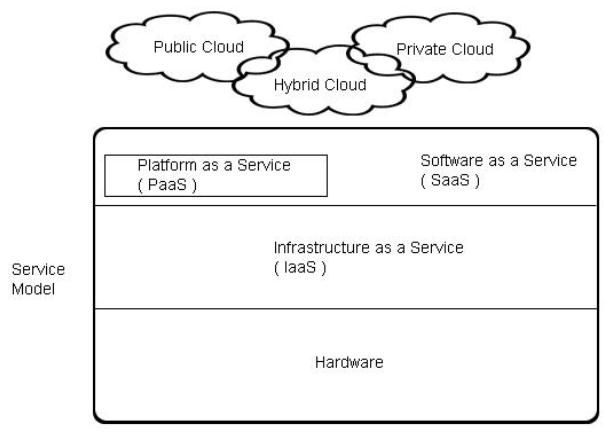
\includegraphics[scale=1]{Gambar35.jpg}\\
\textbf{Gambar 3.5}
\end{center}
\tab \textit{Cloud computing} memberikan banyak keuntungan yang secara umum yaitu dapat ditingkatkan skala pengembangan, dapat dihandalkan, dan keamanan. Sedangkan bagi pengguna memberikan kemudahan dan keuntungan dalam menekan biaya baik dari sisi IT maupun dari sisi operasional.\\
\tab Sedangkan bagi provider memberikan kemudahan bagi pengelolaan, menekan biaya dalam maintenance layanan, memberikan kemudahan dalam melakukan diffrensiasi produk dengan penggunaan SLA, optimasi resource, harga produk atau service yang dijual lebih terjangkau.\\
\tab Karena setiap layanan yang terdapat pada cloud terkait dengan pelayanan public dan bisnis serta teknologi informasi yang menjadi peranan utama ( IT ), maka organisasi ICT ( \textit{information and communication technologies} ) membuat standarisasi yang mengatur pelayanan cloud computing yaitu ITIL V3 dan ISO/IEC 20000 : 2005.\\
\tab Berikut ini adalah beberapa tolak ukur yang digunakan untuk menilai setiap layanan yang diberikan oleh provider cloud berdasarkan ITIL V3 dan ISO/IEC 20000 : 2005\\
\begin{itemize}
\item Konfigurasi manajemen database ( CMDB ) : Pengukuran dilakukan dari sistem database yaitu, Tipe dari database, aplikasi penunjang untuk dapat memodifikasi data dalam database, backup database, relasi atar database tersebut, integrasi database dengan tipe database lain dan mendapatkan bantuan teknis dalam melakukan konfigurasi database.\\
\item \textit{Service level management} : Pengukuran dilakukan dari secara implisit terhadap setiap level dari layanan yang diberikan oleh provider dan pengukuran dimulai dari \textit{SLA ( Service Level Agreement )} yang diberikan oleh provider \textit{service cloud}.
\item \textit{Service continutity} dan \textit{availability management} : Pengukuran dilakukan dari kemudahan dan fleksiblenya layanan yang diberikan oleh provider, baik dari sisi upgrade atau downgrade layanan, dan seberapa lama layanan tersebut sudah dipublikasi dan dijual ke pasaran.
\item \textit{Resolution process} : Pengukuran dilakukan dari kemampuan team manajemen provider dalam menangani berbagai proses seperti \textit{indicents} ( bencana ), \textit{problem technical} ( masalah teknis ) dan tanggapan atas permintaan tertentu atau perubahan tertentu.
\item \textit{Service reporting} : Pengukuran dilakukan dari kemampuan provider dalam menyediakan laporan baik terhadap layanan yang digunakan, laporan historical layanan tersebut digunakan, laporan waktu penggunaan layanan yang dibeli.
\item \textit{Capacity management} : Pengukuran dilakukan atas performance provider baik dari sisi teknis maupun sisi manajemen. Pengukuran ini menghasilkan nilai kemampuan provider dalam memenuhi setiap kebutuhan konsumennya.
\item \textit{Information security management} : Pengukuran dilakukan dari sisi keamanan sistem, jaringan atau network yang tersedia, dan sisi keamanan infrastruktur yang dimiliki oleh provider. Bahkan pengukuran ini dilakukan dari sisi teknologi keamanan data yang dimiliki oleh provider.
\item \textit{Business relationship management} : Pengukuran diukur dari beberapa faktor bisnis yang akhirnya akan memberikan hasil kemampuan provider dalam menfasilitasi dan menyediakan solusi bagi bisnis.
\end{itemize}
Dari beberapa pengukuran seperti yang dijelaskan diatas, maka dapat dikelompokkan dalam beberapa kategori yang dapat diukur :\\
\begin{itemize}
\item \textit{Incident} manajemen : kata \textit{incident} memiliki arti sesuatu hal yang tidak diinginkan dan terjadi dalam waktu yang tidak direncanakan. Konotasi dari \textit{incident} lebih memiliki nuansa negatif. \textit{Incident} manajemen adalah sebuah proses untuk mengatasi dan menangani segala kejadian buruk yang mungkin terjadi, termasuk masalah teknis dan pertanyaan yang diberikan oleh pengguna.\\
Penilaiannya termasuk:
\begin{itemize}
\item Kemampuan untuk mendeteksi dan mengatasi setiap kejadian. Hasilnya berupa nilai / presentasi \textit{downtime}.
\item Kemampuan untuk mengidentifikasi prioritas bisnis secara \textit{realtime} dan pengalokasian sumber daya komputer secara dinamis.
\item Kemampuan untuk mengidentifikasi potensi kejadian yang mungkin terjadi. Hasilnya berupa opini atau rekomendasi solusi.
\item Kemampuan \textit{helpdesk} dalam mengatasi keluhan dan masalah.
\end{itemize}
\item \textit{Change} manajemen : Memastikan setiap perubahan yang terjadi sepengetahuan pengguna, mendapatkan persetujuan, dan dikaji ulang kembali sebelum diimplementasikan oleh pengguna. \textit{Change} manajemen memastikan setiap perubahan yang terjadi dalam pengendalian pengguna. Dapat dilihat pada gambar 3.5.1
\begin{center}
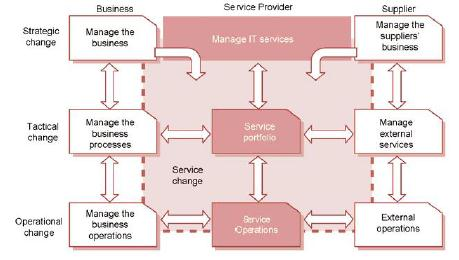
\includegraphics[scale=1]{Gambar351.jpg}\\ 
\textbf{Gambar 3.5.1}
\end{center}
\item \textit{Capacity} manajemen : Memastikan biaya yang dikeluarkan sesuai dan seimbang dengan ukuran atau harapan yang ingin dicapai melalui investasi TI. Pengukuran dilakukan dengan melihat 2 sisi yaitu :
\begin{itemize}
\item Sisi kapasitas bisnis : perencanaan dan kebutuhan bisnis diselaraskan dengan perencanaan TI di kemudian hari. Pengukuran dapat diambil dari beberapa data yang tersedia, layanan TI yang sudah tersedia, dan \textit{forecast} TI. Semua pengukuran tersebut pada dasarnya hanyalah sebuah strategi
\item Sisi kapasitas dalam pelayanan : terfokus pada pelayanan dan pengukuran performance TI yang sedang digunakan, performance operational \textit{helpdesk} TI.
\item Sisi komponen TI : terfokus pada pengendalian, utility, dan performance komponen TI. Dapat dilihat pada gambar 3.5.2.
\begin{center}
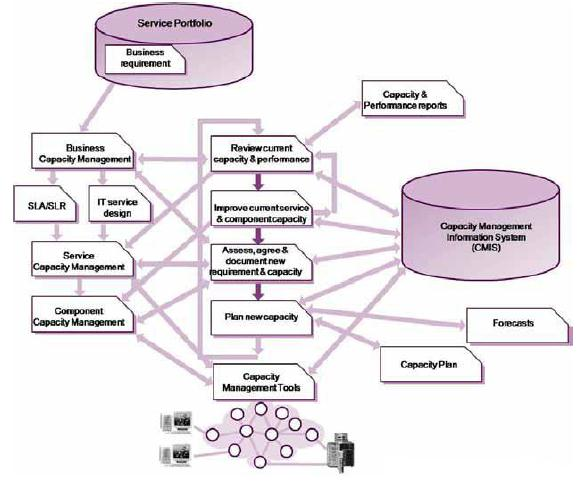
\includegraphics[scale=1]{Gambar352.jpg}\\ 
\textbf{Gambar 3.5.2}
\end{center}
\end{itemize}
\item \textit{Availability} manajemen : Terfokus pada kemampuan manajemen dalam memberikan layanan sesuai dengan kebutuhan dan keinginan pengguna. Dapat dilihat pada gambar 3.5.3
\begin{center}
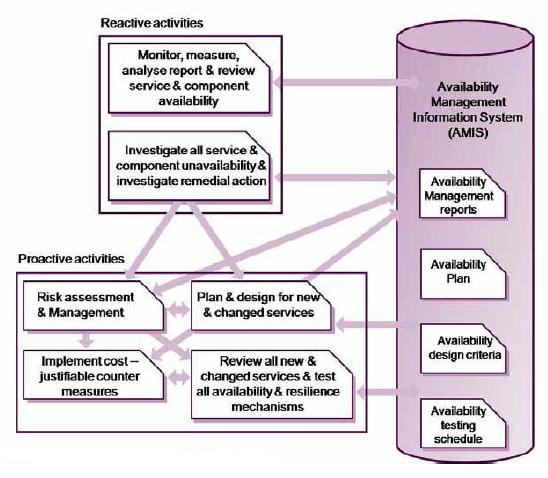
\includegraphics[scale=1]{Gambar353.jpg}\\
\textbf{Gambar 3.5.3}
\end{center}
\item \textit{Problem} manajemen : Terfokus pada usaha untuk meminimalkan akibat dari setiap kejadian, yang akan memberikan hasil kecilnya resiko yang akan ditanggung oleh bisnis. Problem manajemen terkait dengan \textit{change} manajemen setiap kali terjadi perubahan. Dapat dilihat pada gambar 3.5.4.
\begin{center}
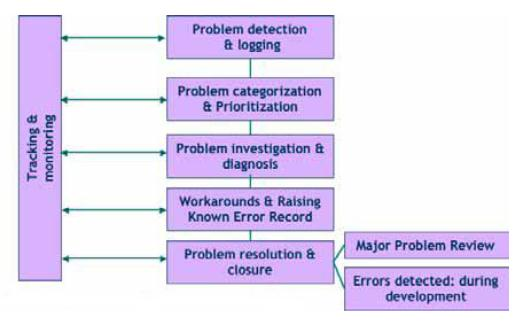
\includegraphics[scale=1]{Gambar354.jpg}\\
\textbf{Gambar 3.5.4}
\end{center}
\textit{Problem} manajemen memiliki beberapa kategori yaitu :
\begin{itemize}
\item \textit{Problem} : Sesuatu kejadian yang belum jelas, biasanya masih dalam tahap investigasi.
\item \textit{Know error} : Sesuatu kejadian yang diketahui penyebabnya, biasanya ini dilakukan setelah selesai mendiagnosis suatu masalah atau \textit{problem}.
\item KEDB : Penyebab error-nya database.
\item \textit{Workaround} : Dokumen teknis yang menjadi acuan user dalam bertindak ketika terjadi masalah.
\end{itemize}
\item \textit{Event} manajemen : Terfokus pada monitoring operasional dan pengendalian
\item \textit{Service} validasi dan \textit{testing} : Memiliki beberapa focus yang ingin diraih, yaitu:
\begin{enumerate}
\item Meningkatkan kepercayaan untuk membuat layanan baru atau mengubah layanan tertentu, meningkatkan nilai jual.
\item Menjadi validasi bahwa service atau layanan sesuai dengan kebutuhan dan keinginan pengguna.
\item Menjamin layanan sesuai dengan kebutuhan dengan menerbitkan \textit{terms and conditions use}.
\end{enumerate}
\end{itemize}
\tab Dari semua faktor pengukuran yang telah diuraikan dan mengacu kepada ITIL V3 dan ISO/IEC 20000:2005, beberapa provider memberikan jasa penilaian terhadap layanan dari provider \textit{cloud} yang lain.\\
\tab Kesimpulan dari \textit{management service process} ( MSP ) : provider cloud tertentu atau \textit{consultant cloud} memberikan jasa penilaian terhadap layanan \textit{cloud computing} yang tersedia di pasaran yang nantinya diselaraskan dengan kebutuhan dan keinginan pengguna atau bisnis, sehingga dengan jasa dari \textit{consultant cloud} ini akan didapatkan hasil layanan \textit{cloud} terbaik yang cocok untuk diimplementasikan dan mendukung kinerja dan produktifitas bisnis.\\
\tab Penilaian yang diberikan oleh \textit{consultant cloud} tentunya mengacu dan berorientasi kepada acuan dari ITIL V3 dan ISO/IEC 20000:2005\\\\
\section{\textit{Integrated Network}}
\tab \textit{Network} atau jaringan merupakan link utama atau jaringan utama yang menghubungkan antara pengguna layanan \textit{cloud} dengan penyedia pusat data dan provider layanan \textit{cloud}. Pada \textit{cloud computing} secara \textit{network} atau jaringan terbagi dalam tiga kategori :\\
\begin{enumerate}
\item \textit{Public Cloud}\\
Suatu model dari layanan \textit{cloud} yang mendeskripsikan layanan \textit{cloud} tersebut menggunakan sumber daya komputerisasi yang ditujukan, didesign dan dapat digunakan secara massal, seperti CPU atau kapasitas penyimpanan dan aplikasi atau software yang tersedia di internet.\\
Banyak provider \textit{cloud} yang menawarkan layanan berbasis \textit{cloud computing} seperti amazon EC2, force.com, google dan provider lainnya.\\
\item \textit{Private Cloud}\\
Suatu model dari layanan \textit{cloud} yang bertolak belakang dengan model \textit{public cloud}, pada model ini lebih terfokus pada kalangan tertentu dan bersifat \textit{private} atau tertutup. Biasanya layanan ini berskala \textit{enterprise}.\\
\textit{Private cloud} juga merupakan model yang merepresentasikan suatu model layanan \textit{cloud} yang bekerja di belakang jaringan atau \textit{network} perusahaan atau kepentingan pribadi user.\\
Ciri khas dari \textit{private cloud} biasanya berupa keharusan untuk membeli atau membayar layanan \textit{cloud} sebelum mencobanya. Ciri khas seperti ini menunjukkan seakan \textit{private cloud} tidak memiliki keunggulan dibandingkan dengan model \textit{cloud} yang lain.\\
Jika dilihat dari kacamata perdagangan, model \textit{private cloud }seakan menjebak konsumen atau sedikit memaksakan konsumen untuk membayar layanan \textit{cloud} tersebut sebelum menggunakannya.\\
Keunggulan dari model \textit{private cloud} adalah model layanan \textit{cloud} yang mendapatkan prioritas dalam pengembangan ( terdepan dalam inovasi ), dan lebih difokuskan kepada kalangan bisnis.\\
\item \textit{Hybrid Cloud}\\
Model yang merepresentasikan campuran antara model \textit{public cloud} dengan model \textit{private cloud}. Model \textit{hybrid cloud} ini merupakan model pengembangan dari layanan \textit{cloud} dimana provider layanan \textit{cloud} mengelola dan menggunakan internal sumber daya komputerisasinya dan menggunakan sumber daya komputerisasi dari provider \textit{cloud} yang lainnya. \\
\end{enumerate}
\textit{Hybrid cloud} memegang peranan utama dalam evolusi generasi baru paradima TI. Pada gambar 3.6 merupakan arsitektur \textit{network} dari \textit{hybrid cloud}.
\begin{center}
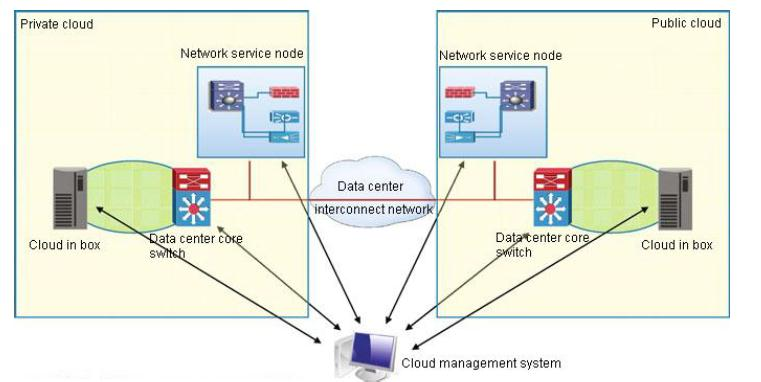
\includegraphics[scale=1]{Gambar36.jpg}\\
\textbf{Gambar 3.6 Arsitektur Network untuk \textit{Hybrid Cloud}}
\end{center}
Gambar 3.6 menjelaskan beberapa komponen utama \textit{network} membentuk suatu jaringan\textit{ private cloud} dan \textit{public cloud}, melalui jaringan \textit{interconnect} maka terjadi penggabungan dua jaringan \textit{cloud} yang berbeda menjadi satu jaringan yang disebut sebagai \textit{hybrid cloud}.\\
\tab Komponen \textit{cloud in box }adalah komponen yang diistilahkan sebagai sel nya \textit{cloud} ( \textit{cloud cell }) berfungsi sebagai \textit{pre-integrated, pre-package} dan secara aktif mengirimkan \textit{service platform} sehingga mudah dan cepat digunakan untuk diimplementasikan dalam jaringan \textit{private} dan \textit{public cloud}.\\
\tab Bentuk fisiknya, berupa \textit{chasis} tunggal layaknya server tetapi memiliki banyak \textit{slot blades ( multiple blades )}, dalam \textit{blade} terdapat beberapa unit komponen komputerisasi, beberapa storage, beberapa processor. \textit{Multiple blade} inilah yang berfungsi untuk \textit{interconnect} semua kombinasi \textit{blade} pada \textit{backplane} dan menyatukan semua koneksi \textit{Ethernet} berkecepatan tinggi ( \textit{high speed} ) yang biasanya berkecepatan 10 gigabyte \textit{fiber optic over Ethernet.}\\
\tab \textit{Core} utama dari software berbasis virtualisasi yaitu \textit{hypervisor}, secara tipikal memiliki kemampuan untuk mengembangkan lingkungan sistemnya melintasi beberapa unit komputerisasi, beberapa unit jaringan atau \textit{networking}, dan beberapa unit \textit{storage} dalam \textit{cloud-in-box}.\\
\tab Dari prespektif \textit{network}, membutuhkan \textit{virtual network switch} yang sudah di-\textit{embeded} ( sudah ditanamkan ) dalam \textit{hypervisor}, seperti yang terlihat pada gambar 3.6.1, sedangkan pada gambar 3.6.2 adalah \textit{ethernet frame} dari \textit{virtual network switch}.\\
\begin{center}
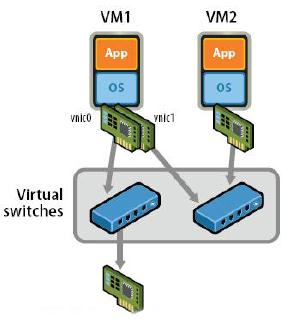
\includegraphics[scale=1]{Gambar361.jpg}\\
\textbf{Gambar 3.6.1 \textit{Virtual Network Switch}}
\end{center}
\begin{center}
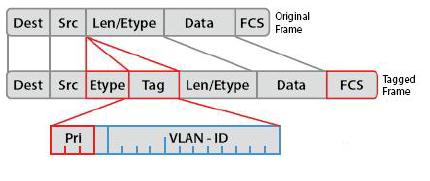
\includegraphics[scale=1]{Gambar362.jpg}\\
\textbf{Gambar 3.6.2}
\end{center}
\tab Komponen \textit{network service node} memegang peranan utama dalam arsitektur \textit{network} dari \textit{hybrid cloud, firewall} pada lapisan ini menjamin keamanan data dalam pengiriman ( \textit{secure transport} ), sedangkan \textit{load balance} pada lapisan ini berfungsi menjaga keseimbangan beban kerja yang terjadi.\\
\tab Manajemen dari \textit{network} arsitektur pada \textit{hybrid cloud} terletak pada \textit{cloud management system}. \textit{Virtual switch} memiliki kemampuan untuk mengimplementasikan aturan keamanan ( \textit{security policies }) ke dalam virtual mesin.\\
\begin{center}
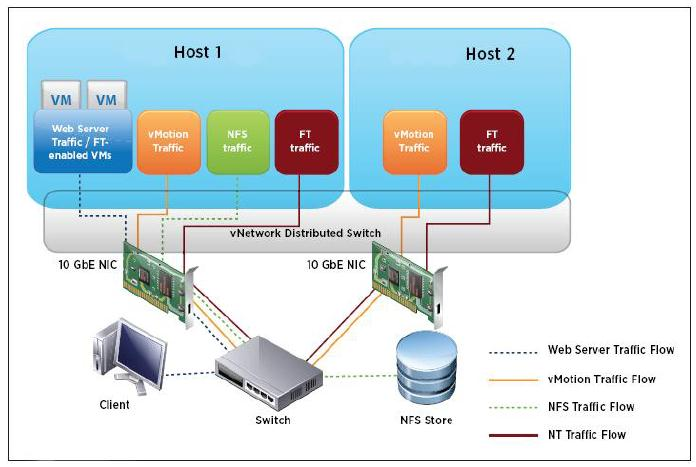
\includegraphics[scale=1]{Gambar363.jpg}\\ 
\textbf{Gambar 3.6.3 \textit{Traffic}}
\end{center}
\tab Pada gambar 3.6.3 menjelaskan aliran \textit{traffic} yang dapat dilakukan oleh \textit{virtual switch}, dimana oleh \textit{vnetwork distributed switch} atau virtual distribusi switch berperan sebagai pengendalian \textit{traffic} dan melakukan pemisahan \textit{traffic} berdasarkan alamat tujuan host.\\
\tab Atas dasar kemampuan dari \textit{vnetwork distributed switch}, maka pemakaian bandwidth menjadi efisien. Gambar 3.6.4 menunjukkan penerapan virtual mesin menggunakan bandwidth yang efisien dalam pemrosesan.\\
\begin{center}
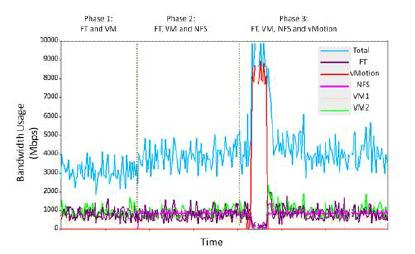
\includegraphics[scale=1]{Gambar364.jpg}\\\textbf{Gambar 3.6.4}
\end{center}
Dengan arsitektur dan kemampuan teknologi virtualisasi, provider cloud menawarkan layanan integrated network kepada pengguna dalam berbagai produk atau layanan :
\begin{itemize}
\item Untuk pengguna ( user ) : \textit{Online storage} atau CloudNAS, VPS ( \textit{virtual private server} )
\item Untuk bisnis : \textit{integrated network, MobileMe iDisk, parallel processing system, automation system, GPS}
\end{itemize}